% !TeX spellcheck = en_US
\documentclass[french]{yLectureNote}

\title{Optique ondulatoire}
\subtitle{Physique}
\author{Paulhenry Saux}
\date{\today}
\yLanguage{Français}

\professor{F.Pettinari}
\usepackage{graphicx}%----pour mettre des images
\usepackage[utf8]{inputenc}%---encodage
\usepackage{geometry}%---pour modifier les tailles et mettre a4paper
%\usepackage{awesomebox}%---pour les boites d'exercices, de pbq et de croquis ---d\'esactiv\'e pour les TP de PC
\usepackage{tikz}%---pour deiffner + d\'ependance de chemfig
% \usepackage{tabularx}%---pour dimensionner automatiquement les tableaux avec variable X
\usepackage{awesomebox}%---Pour les boites info, danger et autres
\usepackage{menukeys}%---Pour deiffner les touches de Calculatrice
\usepackage{fancyhdr}%---pour les en-t\^ete personnalis\'ees
\usepackage{blindtext}%---pour les liens
\usepackage{hyperref}%---pour les liens (\`a mettre en dernier)
\usepackage{caption}%---pour la francisation de la l\'egende table vers Tableau
\usepackage{pifont}
\usepackage{array}%---pour les tableaux
\usepackage{lipsum}
\usepackage{yFlatTable}
\usepackage{multicol}
\newcommand{\Lim}[1]{\lim\limits_{\substack{#1}}\:}
\renewcommand{\vec}{\overrightarrow}
\newcommand{\N}[0]{\mathbb{N}}
\newcommand{\dd}{\mathrm{d}}
\newcommand{\norm}[1]{||\vec{#1}||}
\newcommand{\fo}{\psi(\vec{r},t)}
\newcommand{\foe}{\psi(\vec{r},t)\*}
\newcommand{\HH}{\hat{H}}
\newcommand{\hb}{\hbar}
\newcommand{\lap}{\nabla^2}
\newcommand{\lapcc}{\frac{\partial^2 }{\partial x^2}+\frac{\partial^2 }{\partial y^2}+\frac{\partial^2 }{\partial z^2}}
\newcommand{\mpsi}{\(\psi\)}
\newcommand{\und}{\underline}
\newcommand{\dph}{\Delta\varphi}
\begin{document}
\setcounter{chapter}{1}
\chapter{Interférences d'ondes lumineuses}
\section{Formulaires}
\begin{theorem}[Principe de superposition]
Pour 2 ondes de m\^eme pulsation, on n'additionne pas les intensités I mais les fonctions d'onde.
\end{theorem}

\begin{proposition}[Intensité résultantes du principe de superposition]
Pour \(\und{\fo_1} = \psi_{10}(\vec{r})e^{-i(\omega t + \phi_1(\vec{r}))}\) et

\(\und{\fo_2} = \psi_{20}(\vec{r})e^{-i(\omega t + \phi_1(\vec{r}))}\),

on a \(I(\vec{r}) = I_1(\vec{r})+I_2(\vec{r}) + 2\sqrt{I_1(\vec{r})+I_2(\vec{r})}\cos(\phi_2(\vec{r})-\phi_1(\vec{r}))\) avec \(\Delta \phi = \phi_1-\phi_2\) le terme d'interférence
\end{proposition}

\begin{proposition}[Interférences constructives]
Si \(\cos(\Delta \phi) > 0\), on a des interférences constructives, dans le cas contraire, elles sont destructives.
\end{proposition}

\begin{definition}[Ordre d'interférence]
\(p = \frac{\Delta \phi}{2\pi}\). Quand il est entier, \(I\) est maximal, quand il est demi-entier, \(I\) est minimal
\end{definition}

\begin{definition}[Visibilité]
\[V = \frac{I_{max}-I_{max}}{I_{max}+I_{min}}\]
\end{definition}
\section{Calculs à connaître}
\subsection{2 ondes planes}
On prend \(\und{\fo_1} = \psi_{10}e^{i(\vec{k}\cdot \vec{r}-\omega t+\varphi_1)}\) et \(\und{\fo_2} = \psi_{20}e^{i(\vec{k}\cdot \vec{r}-\omega t+\varphi_2)}\) de m\^eme pulsation,  norme de vecteur d'onde \(k\) mais \(\vec{k_1}\neq \vec{k_2}\)\marginInfo{Ainsi, \(\norm{k_1} = \frac{n\omega}{c} = \norm{k_2}\). Seule la direction change.}.

On a
\explanation{c21}{Le second terme est un décalage uniforme que l'on peut choisir nul}
\explanation{c22}{\(\vec{k}\) est la différence entre les 2 vecteurs d'onde, il vaut ici \(2k\sin(\theta)\vec{e_z}\)}
\begin{flalign*}
\dph &= \phi_2-\phi_1\\
&= (\vec{k_2}\cdot \vec{r}+\varphi_2)- (\vec{k_1}\cdot \vec{r}+\varphi_1)\\
&= (\vec{k_2}- \vec{k_1})\cdot \vec{r}+(\varphi_2-\varphi_1)\explain{c21}{right}{0}{0.5}{}\\
&= 2k\sin(\theta)\vec{e_z}\\
&= \vec{k}\explain{c22}{right}{0}{0.5}{}
\end{flalign*}
On a \[I(\vec{r}) = I_1+I_2+2\sqrt{I_1I_2}\cos(2k\sin(\theta)z)\] On verra donc sur un écran des franges (lignes)\marginWarning{Pour avoir cette distance visible à l'œil nu (i = 1mm) et \(\lambda = 500 nm\), il faut \(\sin(\theta) = 2.5\cdot10^{-5}\). Il faut donc un très petit angle.}


\includegraphics[scale=0.5]{schema3}
\begin{definition}[Interfrange de 2 ondes planes]
C'est la distance entre les franges, notée \(i\) avec \[i = \frac{2\pi}{2k\sin(\theta)} = \frac{\lambda}{2\sin(\theta)}\]
\end{definition}
\subsection{2 ondes sphériques}
\subsubsection{Écran parallèle}
\includegraphics[scale=0.4]{ecran}
% En supposant \(a<< D\) et en  introduisant ici la différence de marche \(\delta\) de 2 ondes on trouve \[\dph = \frac{2\pi}{\lambda_0}\delta\]

On note \(\fo_1 = \frac{A}{r_1}e^{i(kr_1-\omega t-\varphi_1)}\) et  \(\fo_2 = \frac{A}{r_2}e^{i(kr_2-\omega t-\varphi_2)}\)

% L'intensité en M vaut \(I_1 = |\frac{A}{r_1}|^2, I_2 = |\frac{A}{r_2}|^2\) et la différence de phase
On cherche la différence de phase :
\explanation{e1}{On suppose que \(\varphi_2-\varphi_1 = 0\).}
\begin{flalign*}
\Delta \varphi &= (kS_2M-\varphi_2) - (kS_1M-\varphi_1)\\
&= k(S_2M-S_1M)-(\varphi_2-\varphi_1)\\
&= \frac{2\pi}{\lambda_0}n(S_2M-S_1M)\explain{e1}{right}{0}{0.5}{×}\\
&=\frac{2\pi}{\lambda_0}((S_2M)-(S_1M))\\
&=\frac{2\pi}{\lambda_0}(\delta)
\end{flalign*}

\warningInfo{Hypothèse / Simplification}{On suppose que l'écran est loin des sources. Cela amène la simplification suivante : \(D>>a\) et M est proche du centre de l'écran, donc \(D>>x,y\)}

On peut donc prendre \(I_1\simeq I_2 \simeq |\frac{A}{r}|^2 = I_0\).\marginCritical{On ne peut pas faire cette hypothèse pour la phase car elle évolue beaucoup plus rapidement, sur de plus petites distances, à l'échelle de \(\lambda\). Elle se trouve en effet dans un cosinus et est très petite. On garde donc \(r_1\neq r_2\) dans la phase.}

% On a : \(S_1M = \sqrt{x^2+y²2+(z-\frac{a}{2})^2}\) et \(S_2M = \sqrt{x^2+y²2+(z+\frac{a}{2})^2}\).
On calcule \(S_1M\) :
\explanation{s1}{
C'est ici que l'on utilise l'hypothèse : on a toujours \(D >>y,z\), donc on peut écrire que, donc on peut utiliser le DL \((1+\epsilon)^{1/2}\) à l'ordre 1}
\begin{flalign*}
S_1M &= \sqrt{D^2+y^2+(z-\frac{a}{2})^2}\\
&=  (D^2(1+\frac{y^2}{D^2}+\frac{(z-a/2)^2}{D^2}))^{\frac12}\\
&\simeq D(1+\frac{y^2}{2D^2}+\frac{(z-a/2)^2}{2D^2})\explain{s1}{right}{0}{0.5}{}
\end{flalign*}

De m\^eme pour \(S_2M\) : \[S_2M \simeq D(1+\frac{y^2}{2D^2}+\frac{(z+a/2)^2}{2D^2})\]

On peut maintenant calculer la différence de marche \(\delta\) :
\begin{flalign*}
\delta &= n(r_2-r_1)\\
&= \frac{n}{2D}((z+a/2)^2-(z-a/2)^2)\\
&= \frac{naz}{D}\\
\Delta \varphi &= \frac{2\pi az}{\lambda D}
\end{flalign*}
On en déduit l'intensité en M :
\begin{flalign*}
I_M  &= I_1+I_2+2\sqrt{I_1I_2}\cos(\Delta \phi)\\
&= I_0+I_0+2\sqrt{I_0^2}\cos(\Delta \phi)\\
&= 2I_0+I_0\cos(\Delta \phi)\\
I_M  = 2I_0(1+\cos(\frac{2\pi az}{\lambda D}))
\end{flalign*}
\begin{proposition}[Intensité d'interférence sur un tableau]
\[I_M  = 2I_0(1+\cos(\frac{2\pi az}{\lambda D}))\]
\end{proposition}

On cherche maintenant l'Interfrange i (période spatiale de l'interférogramme) : \(i = \frac{\lambda D}{a}\)\marginCheck{Pour l’observer, il faut que i soit de l'ordre du mm. En prenant \(\lambda = 500 nm\), donc \(\frac{D}{a} \simeq 10^{3}\), donc \(a\simeq 1mm\)}
\subsubsection{Écran perpendiculaire}
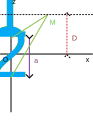
\includegraphics[scale=0.5]{schema6}

On suppose également l'écran loin des sources et M proche du centre.

On trouve que \(\delta = na(1-\frac{x^2+y^2}{2D^2})\) et \(\Delta \varphi  = \frac{2\pi}{\lambda_0}na(1-\frac{x^2+y^2}{2D^2})\). On en déduit \(I(M) = 2I_0(1+\cos(\frac{2\pi}{\lambda_0}na(1-\frac{x^2+y^2}{2D^2})))\)

La forme géométrique de l'interférogramme (lieux d'égale intensité). On cherche donc \(\Delta \varphi = Cst \iff x^2+y^2 = Cst\) qui est l'équation d'un cercle centré au centre de l'écran.


Dans cette configuration, l'écran est perpendiculaire à l'axe joignant les deux sources \(S_1\) et \(S_2\). On suppose que les sources sont situées sur l'axe des \(x\) en \(S_1 = (-a/2, 0, 0)\) et \(S_2 = (a/2, 0, 0)\). L'écran est un plan situé à une distance \(D\) des sources, donc dans le plan d'équation \(x=D\). Un point \(M\) sur l'écran a les coordonnées \((D, y, z)\).

Le calcul de la \textbf{différence de marche optique} \(\delta\) nécessite de déterminer les distances \(S_1M\) et \(S_2M\) en utilisant le théorème de Pythagore dans l'espace.
\begin{flalign*}
S_1M &= \sqrt{(D - (-a/2))^2 + (y-0)^2 + (z-0)^2} = \sqrt{(D+a/2)^2 + y^2 + z^2} \\
S_2M &= \sqrt{(D - a/2)^2 + (y-0)^2 + (z-0)^2} = \sqrt{(D-a/2)^2 + y^2 + z^2}
\end{flalign*}

\warningInfo{Hypothèse}{On utilise les m\^emes hypothèses que précédemment}

On utilise l'approximation du développement limité à l'ordre 1 pour \(\sqrt{1+\epsilon} \simeq 1+\epsilon/2\).
\begin{flalign*}
S_1M &= \sqrt{x^2+y^2 + (D-\frac{a}{2})^2}\\
&= (D-\frac{a}{2})\sqrt{1 + \frac{y^2 + x^2}{(D-\frac{a}{2})^2}} \\
&\simeq (D-\frac{a}{2}) + \frac{y^2 + x^2}{2(D-\frac{a}{2})^2}\\
&= D - \frac{a}{2} + \frac{y^2+x^2}{2(D-\frac{a}{2})^2}
\end{flalign*}
De même pour \(S_2M\) :
\begin{flalign*}
S_2M \simeq D + \frac{a}{2} + \frac{y^2+x^2}{2(D+\frac{a}{2})^2}
\end{flalign*}

Calculons la différence de marche \(\delta = n(S_2M - S_1M)\) :
\begin{flalign*}
\delta &= n\left[ a +\frac{x^2+y^2}{2}(\frac{1}{D+\frac{a}{2}}-\frac{1}{D-\frac{a}{2}}) \right] \\
&= n\left[ a +\frac{x^2+y^2}{2}(\frac{(D-\frac{a}{2})-(D+\frac{a}{2})}{D^2-\frac{a^2}{4}}) \right] \\
&= n\left[ a +\frac{x^2+y^2}{2}(\frac{-a}{D^2-\frac{a^2}{4}}) \right] \\
&= n\left[ a +\frac{x^2+y^2}{2}(\frac{-a}{D^2}) \right] \\
&= na(1-\frac{x^2+y^2}{2D^2})
\end{flalign*}
La différence de phase vaut alors \[\Delta \phi = 2\pi \frac{na}{\lambda_0}(1-\frac{x^2+y^2}{2D^2})\]

Les lignes d'égale intensité correspondent à \(\Delta\varphi = \text{constante}\).
\[1 - \frac{y^2+x^2}{2D^2} = \text{constante}\]
\[\frac{y^2+x^2}{2D^2} = \text{constante}\]
\[y^2+x^2 = \text{constante}\]
Cette équation représente un cercle centré à l'origine \((y, x)=(0,0)\) de l'écran. L'interférogramme prend donc la forme d'anneaux concentriques. Ce type de franges circulaires est typique des interférences localisées à l'infini ou des franges d'égale inclinaison, comme celles observées avec un Michelson lorsque les miroirs sont parfaitement parallèles.


 \end{document}
